Una partícula con carga positiva se suelta entre
dos placas planas, verticales y electrizadas, como muestra la figura de este problema. Considerando que el peso de la partícula no es despreciable, la trayectoria que describiría corresponde a una de las siguientes. Indíquela.
\begin{figure}[h!]
  \centering
  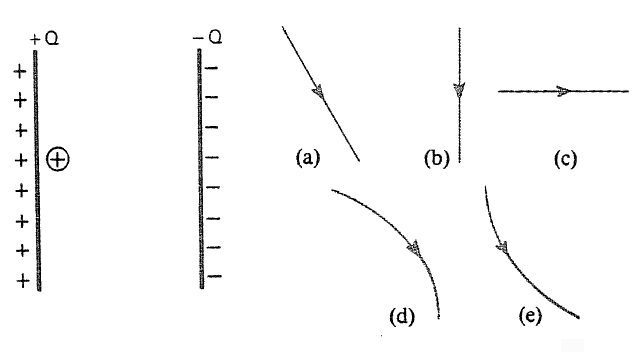
\includegraphics[scale=0.5]{figuras/fig_alvarenga_p861_10.png}
  \caption{Problema 22}
\end{figure}